
\documentclass[a4paper, 11pt, DIV=14]{scrartcl}

\author{Bastian Dittmar}
\date{\today}
\subject{Self Driving Car Nano Degree}
\title{Behavioral Cloning Project}

\usepackage{graphicx}
\usepackage[english]{babel}
\usepackage[utf8]{inputenc}
\usepackage[T1]{fontenc}
\usepackage{lmodern}
\usepackage{microtype}
\usepackage{csquotes}
\usepackage{hyperref}
\hypersetup{
     colorlinks   = true,
     citecolor    = blue,
     linkcolor    = blue
}
\usepackage{amsmath}
\usepackage{listings}

\usepackage[style=authoryear, citestyle=authoryear-icomp, giveninits=true, autolang=hyphen, hyperref=true, minbibnames=3, dashed=false, doi=false, isbn=false, url=false, sorting=nyt, backend=biber]{biblatex}
\setlength{\bibitemsep}{0.5\baselineskip}
\addbibresource{library.bib}

\pagestyle{plain}
\begin{document}
\maketitle


\section{Introduction}
In this project, an end-to-end network is designed using the keras framework and trained to output a steering angle based on an imput image. The input is what a car sees in frot of it using a virtual camera while driving down a given track. The steering angle output will be transmitted to the car and effects its direction directly.
\parencite{LeNet, AlexNet, Yadav, NVidia}

The goals / steps of this project are the following:
\begin{itemize}
\item Use the simulator to collect data of good driving behavior
\item Build, a convolution neural network in Keras that predicts steering angles from images
\item Train and validate the model with a training and validation set
\item Test that the model successfully drives around track one without leaving the road
\item Summarize the results with a written report
\end{itemize}


\section{Files Submitted \& Code Quality}

\subsection{Submission includes all required files and can be used to run the simulator in autonomous mode}

My project includes the following files:
\begin{itemize}
\item model.py containing the script to create and train the model
\item drive.py (unmodified) for driving the car in autonomous mode
\item model.h5 containing a trained convolution neural network
\item test\_drive.mp4 showing the car driving around the track successfully
\item writeup\_report.pdf summarizing the results
\end{itemize}

\subsection{Submission includes functional code}
Using the Udacity provided simulator and my drive.py file, the car can be driven autonomously around the track by executing 

\begin{lstlisting}[language=bash]
  $ sh python drive.py model.h5
\end{lstlisting}

\subsection{Submission code is usable and readable}
The model.py file contains the code for training and saving the convolution neural network. The file shows the pipeline I used for training and validating the model, and it contains comments to explain how the code works. The program executes different actions based on command line parameters. The basic modes are training a network, evaluating a set of images, plotting the accumulated training history and testing the data augmentation.

\section{Model Architecture and Training Strategy}

\subsection{An appropriate model architecture has been employed}

My model is the based on the one used by \textcite{NVidia} from Nvidia, except for the input dimensions and a preprocessing layer. The layers are depicted in figure \ref{fig:network} (implementation in model.py lines 253-305).

The first two layers are for preprocessing. At first a lambda layer scales and shifts the data from an interval of [0, 255] to [-1, +1]. The second layer crops the image remove the bottom 25 and the top 70 pixels. That basically cuts hoff the hood and the sky down to the horizon. At first I applied those two layers the other way around as it should be more efficient to crop first but the network converged worse on my first initial tests. That is wh I went back to this order and never tried again. In principal it should not make a difference regarding the accuracy.

The 5 layers are convolutional layers. Three of them with a kernel size of $5x5$ and a stride of $2x2$ with a growing depth. The last two of the convolutional layers have a kernel size of $3x3$ and a stride of $1x1$. Each convolutional layer is followed by a relu activation to introduce non-linearity.

Next the network is flattened and the data passed through four fully connected layers reducing the output to 100, 50, 10 and 1 where the last one is the output of the network and thus the steering angle to be learned.

\begin{figure}
  \centering
    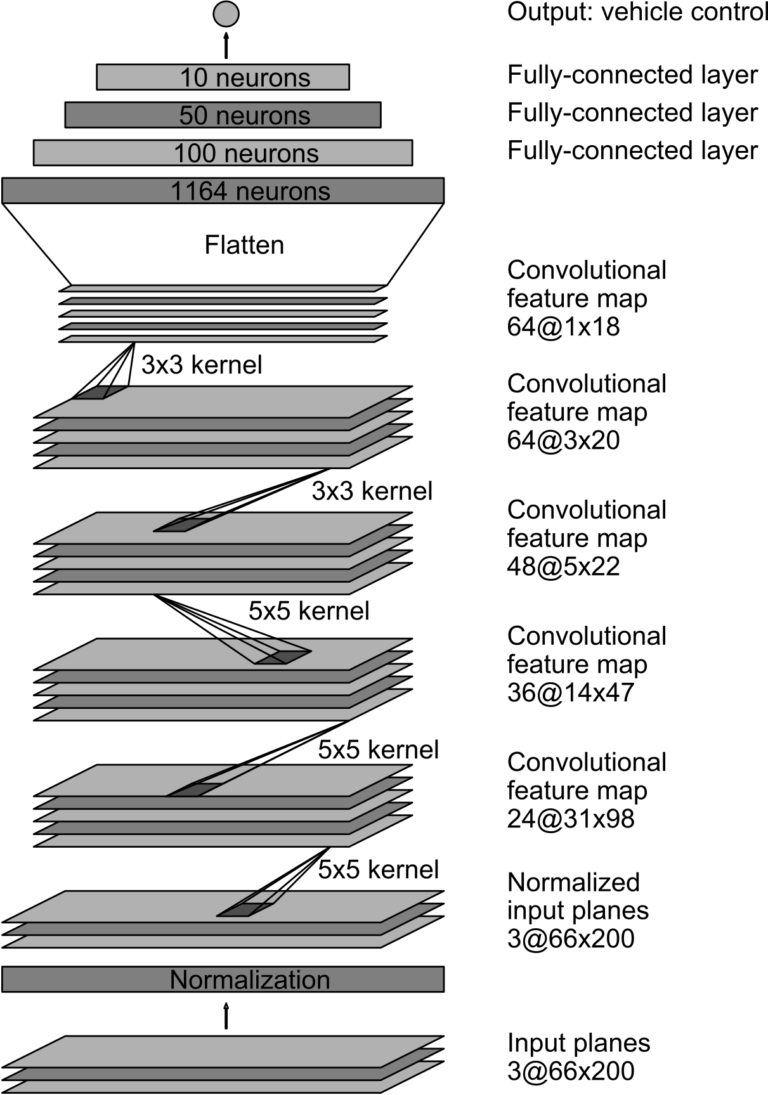
\includegraphics[width=0.5\textwidth]{images/cnn-architecture.png}
    \caption{The network architecture used by \parencite{NVidia}}
    \label{fig:network}
\end{figure}

\subsection{Attempts to reduce overfitting in the model}

The model itself does not contain any specific elements to prevent overfitting as I never ran into any indications of overfitting data.

The model was trained and validated on different data sets to ensure that the model was not overfitting. To gather two distinct sets the training data was split randomly (code line 358). The proportion of validation samples can be set via applicationparameter (--validation_size). For the whole training a factor of 0.2 was used. 

The model was tested by running it through the simulator and ensuring that the vehicle could stay on the track.

\subsection{Model parameter tuning}

The model used an adam optimizer, so the learning rate was not tuned manually (model.py line 304). As a loss function mse was used. which is appropriate for an end-to-end network.

\subsection{Appropriate training data}

Training data was chosen to keep the vehicle driving on the road. I used a combination of center lane driving, recovering from the left and right sides of the road ... 

For details about how I created the training data, see the next section. 

\section{Model Architecture and Training Strategy}

\subsection{Solution Design Approach}

The overall strategy for deriving a model architecture was to ...

My first step was to use a convolution neural network model similar to the ... I thought this model might be appropriate because ...

In order to gauge how well the model was working, I split my image and steering angle data into a training and validation set. I found that my first model had a low mean squared error on the training set but a high mean squared error on the validation set. This implied that the model was overfitting. 

To combat the overfitting, I modified the model so that ...

Then I ... 

The final step was to run the simulator to see how well the car was driving around track one. There were a few spots where the vehicle fell off the track... to improve the driving behavior in these cases, I ....

At the end of the process, the vehicle is able to drive autonomously around the track without leaving the road.

\subsection{Final Model Architecture}

The final model architecture (model.py lines 18-24) consisted of a convolution neural network with the following layers and layer sizes ...

Here is a visualization of the architecture (note: visualizing the architecture is optional according to the project rubric)



\subsection{Creation of the Training Set \& Training Process}

To capture good driving behavior, I first recorded two laps on track one using center lane driving. Here is an example image of center lane driving:

![alt text][image2]

I then recorded the vehicle recovering from the left side and right sides of the road back to center so that the vehicle would learn to .... These images show what a recovery looks like starting from ... :

![alt text][image3]
![alt text][image4]
![alt text][image5]

Then I repeated this process on track two in order to get more data points.

To augment the data sat, I also flipped images and angles thinking that this would ... For example, here is an image that has then been flipped:

![alt text][image6]
![alt text][image7]

Etc ....

After the collection process, I had X number of data points. I then preprocessed this data by ...


I finally randomly shuffled the data set and put Y\% of the data into a validation set. 

I used this training data for training the model. The validation set helped determine if the model was over or under fitting. The ideal number of epochs was Z as evidenced by ... I used an adam optimizer so that manually training the learning rate wasn't necessary.


\printbibliography
\end{document}
